%% 
%% Copyright 2007, 2008, 2009 Elsevier Ltd
%% 
%% This file is part of the 'Elsarticle Bundle'.
%% ---------------------------------------------
%% 
%% It may be distributed under the conditions of the LaTeX Project Public
%% License, either version 1.2 of this license or (at your option) any
%% later version.  The latest version of this license is in
%%    http://www.latex-project.org/lppl.txt
%% and version 1.2 or later is part of all distributions of LaTeX
%% version 1999/12/01 or later.
%% 
%% The list of all files belonging to the 'Elsarticle Bundle' is
%% given in the file `manifest.txt'.
%% 

%% Template article for Elsevier's document class `elsarticle'
%% with numbered style bibliographic references
%% SP 2008/03/01

\documentclass[review]{elsarticle}

%% Use the option review to obtain double line spacing
%% \documentclass[authoryear,preprint,review,12pt]{elsarticle}

%% Use the options 1p,twocolumn; 3p; 3p,twocolumn; 5p; or 5p,twocolumn
%% for a journal layout:
%% \documentclass[final,1p,times]{elsarticle}
%% \documentclass[final,1p,times,twocolumn]{elsarticle}
%% \documentclass[final,3p,times]{elsarticle}
%% \documentclass[final,3p,times,twocolumn]{elsarticle}
%% \documentclass[final,5p,times]{elsarticle}
%% \documentclass[final,5p,times,twocolumn]{elsarticle}

%% For including figures, graphicx.sty has been loaded in
%% elsarticle.cls. If you prefer to use the old commands
%% please give \usepackage{epsfig}

%% The amssymb package provides various useful mathematical symbols
\usepackage{amssymb}
%% The amsthm package provides extended theorem environments
%% \usepackage{amsthm}

%% The lineno packages adds line numbers. Start line numbering with
%% \begin{linenumbers}, end it with \end{linenumbers}. Or switch it on
%% for the whole article with \linenumbers.
%% \usepackage{lineno}

\usepackage{fixltx2e}
\usepackage{diagbox}
\usepackage{makecell}
\usepackage{algorithm,algpseudocode}
\usepackage[flushleft]{threeparttable}
\usepackage{booktabs}
\usepackage{multirow}
\usepackage{colortbl}
\usepackage[table*]{xcolor}
\xdefinecolor{gray95}{gray}{0.45}
\xdefinecolor{gray25}{gray}{0.85}
\xdefinecolor{gray50}{gray}{0.65}
\usepackage{todonotes}
\PassOptionsToPackage{hyphens}{url}\usepackage{hyperref}
\usepackage{epstopdf}
\usepackage[normalem]{ulem}
\usepackage{graphicx}

\usepackage{natbib}



%\newcommand{\markus}[1]{\textcolor{red}{\em #1}}

\usepackage{amsmath} \DeclareMathOperator*{\argmax}{\arg\!\max}

%added by Markus
\newcommand{\markus}[1]{\textcolor{orange}{\em (#1)}}

\newcommand{\ignore}[1]{}

%added by shahriar
\newcommand{\shahriar}[1]{\textcolor{red}{\em (#1)}}
%added by shahriar
\newcommand{\shahriarinline}[1]{\textcolor{blue}{\em #1}}

\usepackage{amsthm}
\theoremstyle{definition}
\newtheorem{definition}{Definition}

\journal{Applied Soft Computing}
\begin{document}

\begin{frontmatter}

%% Title, authors and addresses

%% use the tnoteref command within \title for footnotes;
%% use the tnotetext command for theassociated footnote;
%% use the fnref command within \author or \address for footnotes;
%% use the fntext command for theassociated footnote;
%% use the corref command within \author for corresponding author footnotes;
%% use the cortext command for theassociated footnote;
%% use the ead command for the email address,
%% and the form \ead[url] for the home page:
%% \title{Title\tnoteref{label1}}
%% \tnotetext[label1]{}
%% \author{Name\corref{cor1}\fnref{label2}}
%% \ead{email address}
%% \ead[url]{home page}
%% \fntext[label2]{}
%% \cortext[cor1]{}
%% \address{Address\fnref{label3}}
%% \fntext[label3]{}

\title{Incorporating Domain Knowledge into the Optimization of Energy Systems}

%% use optional labels to link authors explicitly to addresses:
%% \author[label1,label2]{}
%% \address[label1]{}
%% \address[label2]{}

\author[FBK,Unitn]{Md Shahriar Mahbub\corref{cor1}}
\ead{mahbub@fbk.eu}
\author[Adl]{Markus Wagner}
\ead{markus.wagner@adelaide.edu.au}
\author[FBK]{Luigi Crema}
\ead{crema@fbk.eu}

\address[FBK]{Fondazione Bruno Kessler, Via Sommarive 18, 38123 Povo, Trento, Italy.}
\address[Unitn]{University of Trento, Via Sommarive 9, 38123 Povo, Trento, Italy.}
\address[Adl]{University of Adelaide, Adelaide, SA 5005, Australia.}
\cortext[cor1]{Corresponding author}

\end{frontmatter}

\section{Diversity maximization}

\section{results}
In this section we compare the results obtained by smart initialization (SI) technique proposed in the paper and our newly proposed technique which we called diversity maximization (MD).

The figure shows that the proposed technique has very similar results for all indicators. Table~\ref{table:wilcox test SM} also supports the fact that the the samples are statistically insignificant. Therefor, we can conclude that these two techniques produce very similar results. However, time consumption of proposed technique is very good (see Table~\ref{Table:time-consuption}). 

\begin{figure}[h]
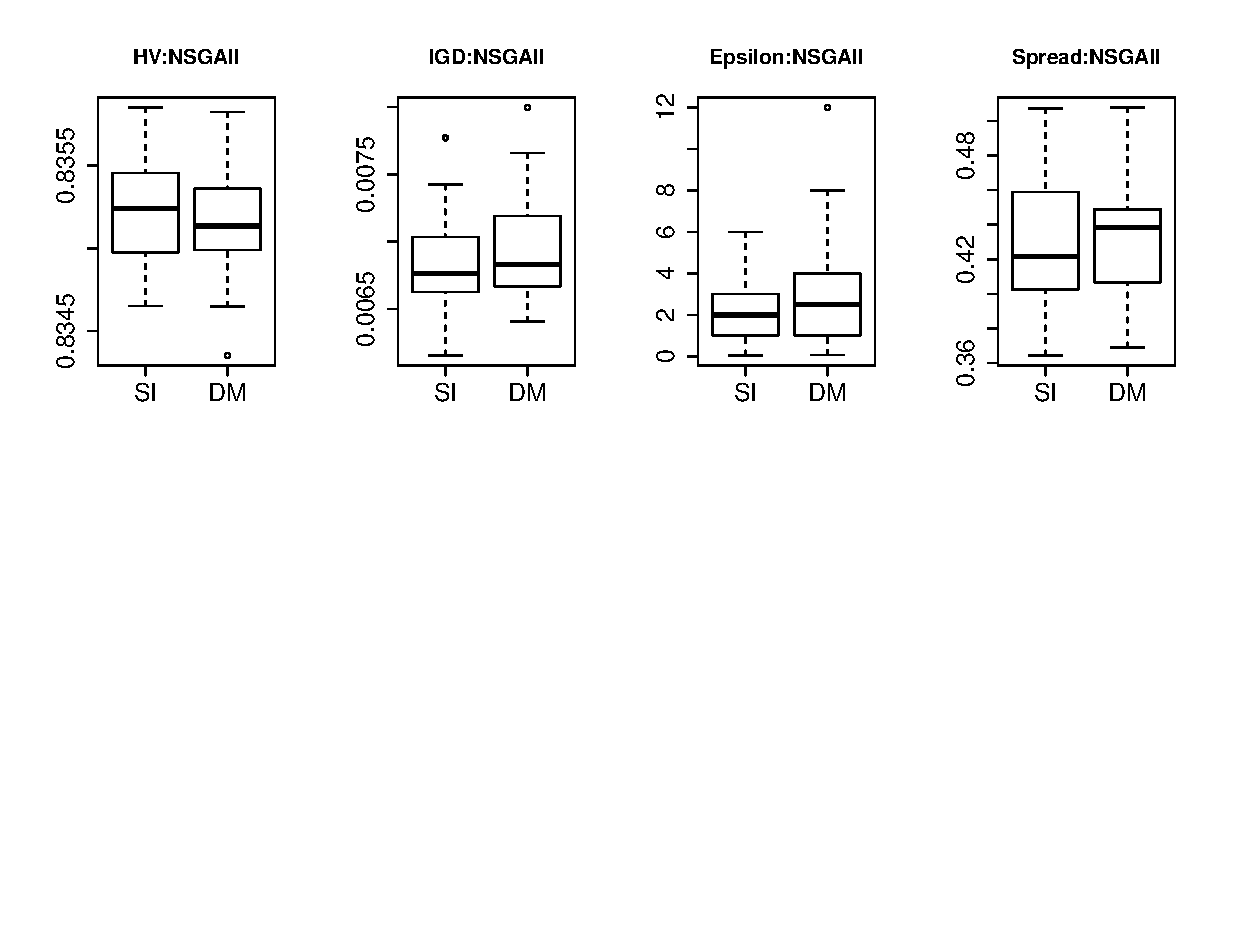
\includegraphics[scale=0.60]{Compare_SI_DivMax.eps}
\end{figure}

\begin{table}[h]
\centering
\caption{Mann-Whitney U-tests: p-values for different metrics when comparing our smart initialization (SI) with the siversity maximization (DM).}
\label{table:wilcox test SM}
\begin{scriptsize}

\begin{tabular}{c|c|c}\hline
\multicolumn{1}{l}{}          & \multicolumn{2}{c}{p-value}                                                                                                                                                                                         \\
\multicolumn{1}{l}{{\begin{tabular}[c]{@{}l@{}}Evaluation \\ metrics\end{tabular}}}& \multicolumn{1}{l}{\begin{tabular}[c]{@{}l@{}}Compare NSGA-II: \\ With SI and DM\end{tabular}} & \multicolumn{1}{l}{\begin{tabular}[c]{@{}l@{}}Compare SPEA2: \\ With SI and DM\end{tabular}} \\ \hline
HV                            & $0.4147$
                                                                                                 & $0.5229$ \\
IGD                           & $ 0.2861$ & $0.9824$
 \\
Epsilon                       & $0.2843$ & $ 0.433$ \\
Spread                        & $0.6865$                                                                                                & $0.1774$ \\ \hline 
\end{tabular}
 
\end{scriptsize}
\end{table}
\begin{table}
\centering
\caption{Time required in seconds}
\label{Table:time-consuption}
\begin{tabular}{c|c}\hline
Technique & time \\ \hline
Smart initialization (prposed in paper) & 8280 \\
Diversity Maximization (proposed here) & 2.18 \\ \hline


\end{tabular}
\end{table}

\section*{Bibliography}
%\bibliographystyle{abbrvnat} % sorts the entries alphabetically, which is different from what the elsarticle-num style is doing (which lists them in the order of citation)
\bibliographystyle{ieeetr} % based on http://tex.stackexchange.com/questions/5053/is-it-possible-to-get-unsrt-abbrv-bibliography
%\bibliographystyle{elsarticle-num} 
\bibliography{els_bibdatabase}

\end{document}
\endinput
%%
%% End of file `elsarticle-template-num.tex'.
